\documentclass[hidelinks, letterpaper,11pt,headheight=10mm]{texMemo}

\usepackage{graphicx}
\usepackage{fancyhdr}
\usepackage{color}
\usepackage{hyperref}
\usepackage{float}
\usepackage{indentfirst}
\usepackage{booktabs, multirow} % for borders and merged ranges
\usepackage{soul}% for underlines
\usepackage{xcolor,colortbl} % for cell colors
\usepackage{changepage,threeparttable} % for wide tables
\usepackage{siunitx}

% Define PSU official colors
% https://www.rri.pdx.edu/files/758/psu_identity_standardscolors.pdf
\definecolor{PSUgreen}{RGB}{106,127,16}
\definecolor{PSUltgreen}{RGB}{168,180,0}
\definecolor{PSUblue}{RGB}{0,117,154}
\definecolor{PSUltblue}{RGB}{161,216,224}
\definecolor{PSUgray}{RGB}{71,67,52}
\definecolor{PSUBrown}{RGB}{96,53,29}
\definecolor{PSUsienna}{RGB}{163,63,31}
\definecolor{PSUred}{RGB}{210,73,42}
\definecolor{PSUorange}{RGB}{220,155,50}
\definecolor{PSUyellow}{RGB}{230,220,143}
\definecolor{PSUtan}{RGB}{232,221,162}
\definecolor{PSUpurple}{RGB}{101,3,96}

%----------------------------------------------------------------------------------------
%    To:/From:
%----------------------------------------------------------------------------------------

\memoto{Jeff Dinsmore, Bob Bass}
\memofrom{William Jeffreys, Greyland Miller, Rodney Downer}
\memosubject{Lab 1 Report Submission}
\memodate{2026-10-16}
\geometry{headheight=60pt, headsep=15pt, includehead}
\setlength{\parindent}{2em} % Increases the first-line indent to 2em (or use 2cm, 20pt, etc.)

\begin{document}
\pagenumbering{arabic}

%----------------------------------------------------------------------------------------
%    Header
%----------------------------------------------------------------------------------------
\pagestyle{fancy}

\fancyhead[L]{\footnotesize\textcolor{PSUgray}{Department of Electrical \& Computer Engineering \\1900 SW 4th Ave, suite 160 \\ Portland, OR 97201}}
\fancyhead[R]{
\includegraphics[width=3in]{psulogo_horiz.png}}
\headrule{\hrule}{\color{PSUgreen}\hrule}{}{}
\renewcommand{\headrulewidth}{0.4pt}

%----------------------------------------------------------------------------------------
%    Footer
%----------------------------------------------------------------------------------------
\footrule{\hrule}{\color{PSUgreen}\hrule}{}{}
\renewcommand{\footrulewidth}{0.4pt}
\fancyfoot[L]{\footnotesize\color{PSUgray}\sffamily
	\href{https://www.pdx.edu/electrical-computer-engineering/power-engineering-focus}{Power Engineering Laboratory} \textbullet\ Fourth Avenue Building, 1900 SW 4$^{th}$ Ave, suite 25-00, Portland, OR 97201}%\fancyfoot[C]{~}
\fancyfoot[R]{\footnotesize~\newline\color{PSUgray}\sffamily\thepage}

\maketitle

\section{Introduction}
The main focus of this lab was to practice the process of power factor (PF) correction. The point of PF correction is to add capacitors to an inductive load, or vice versa, to reduce reactive power transfer from the source to the load.
This affects the magnitude of line current, making it an important technique in regards to efficiency, and reducing the wear and tear on power infrastructure.

\section{Circuit Build \& Data Collection}
\paragraph{}To demonstrate how power factor correction works we will
set up two different circuits.
The first will contain a purely resistive load of 600$\Omega$ and
should therefore have a power factor of 1.
And the second circuit will have a complex load with an inductive
impedance of 300+j300$\Omega$.
With each circuit we will connect a parallel capacitive impedance of
8 specific values, -[171, 200, 240, 300, 400, 600, 1200]$\Omega$.
During the build of the circuit we had an easier time getting
everything connected than we did  the previous lab. One main point of
improvement came when switching between the two circuits. For this we
learned how we could essentially shift all connection up by one,
making the load changes easier.

\paragraph{}With both circuits we measured the line voltage, phase
voltage, line current, the real and reactive power,
and the power factor. Samples were captured for all 8 capacitive
loads. In addition, we calculated theoretical
values for all the same loads. We also calculated these values by
hand using the equations listed bellow in section 2.1.
This allowed us to compare the measured values to expected values.

\clearpage
\subsection{Methods of Calculation}
\begin{itemize}
  \item $\bar{Z}_\|$ - Resulting parallel impedance after adding the
    capacitive load
    \begin{center}
      $\bar{Z}_{\|} = \frac{
        \bar{Z}_{1}\bar{Z}_{2}
      }{
        \bar{Z}_1 + \bar{Z}_2
      }$
    \end{center}

  \item $\bar{I}_L$ - Line current in the phase
    \begin{center}
      $\bar{I}_{L} = \frac{
        V_{\phi}
      }{
        \bar{Z_{\|}}
      }$
    \end{center}

  \item $\bar{S}$ - Complex power in VA
    \begin{center}
      $\bar{S} = 3V_{\phi}I_{L}^*$
    \end{center}

  \item $P$ - Real power in W
    \begin{center}
      $P = \Re(\bar{S})$
    \end{center}

  \item $Q$ - Reactive power in var
    \begin{center}
      $Q = \Im(\bar{S})$
    \end{center}

  \item $\theta$ - Power factor angle
    \begin{center}
      $\theta = \arg(\bar{S})$
    \end{center}

  \item PF - Power factor
    \begin{center}
      PF = $\cos(\theta)$
    \end{center}

  \item PF$_{c}$ - Power factor calculated from measured P, Q
    \begin{center}
      PF$_{c}  = \frac{
        P_{m}
      }{
        |P_{m} + jQ_{m}|
      }$
    \end{center}

  \item $\theta_{m}$ - Power factor angle calculated from the
    measured power factor
    \begin{center}
      $\theta_{m} = \arccos($PF$_{m})$
    \end{center}

  \item
    $\theta_{c}$ - Power factor angle derived from measured $P$ and $Q$
    \begin{center}
      $\theta_{c} = \arctan2(P, Q)$
    \end{center}

\end{itemize}

\clearpage


\section{Data Analysis}
\begin{table}[H]\centering
	\begin{threeparttable}
		\caption{Measured Values}\label{tab:meas}
		\scriptsize
		\setlength{\tabcolsep}{3pt}
		\begin{tabular}{*{12}{r}}\toprule
			\textbf{$V_{LL}$ (V)} & \textbf{$V_\phi$ (V)} & \textbf{$I$ (A)} & \textbf{$Z_1$ ($\Omega$)} & \textbf{$Z_2$ ($\Omega$)} & \textbf{$Z_\|$ ($\Omega$)} & \textbf{$P$ (W)} & \textbf{$Q$ (VAR)} & \textbf{PF$_m$} & \textbf{$\theta_{m}$ ($^\circ$)} & \textbf{PF$_c$} & \textbf{$\theta_{c}$ ($^\circ$)} \\\midrule
			208.2                 & 120.8                 & 0.201            & 600                       & 0                         & 600                        & 72.47            & -0.118             & 0.866           & 30.                              & 1               & 0.1                              \\
			208.2                 & 120.6                 & 0.762            & 600                       & -j171                     & 45.07-j158.2               & 73.06            & -253.1             & 0.693           & 46.13                            & 0.28            & 74.                              \\
			208.1                 & 120.5                 & 0.662            & 600                       & -j200                     & 60-j180                    & 72.47            & -215.4             & 0.715           & 44.36                            & 0.32            & 71.4                             \\
			208.3                 & 120.7                 & 0.562            & 600                       & -j240                     & 82.76-j206.9               & 72.92            & -181               & 0.757           & 40.8                             & 0.37            & 68.                              \\
			208.2                 & 120.6                 & 0.468            & 600                       & -j300                     & 120-j240                   & 72.84            & -144.4             & 0.803           & 36.58                            & 0.45            & 63.2                             \\
			208.1                 & 120.5                 & 0.382            & 600                       & -j400                     & 184.6-j276.9               & 72.02            & -109.1             & 0.851           & 31.68                            & 0.55            & 56.57                            \\
			208.2                 & 120.6                 & 0.297            & 600                       & -j600                     & 300-j300                   & 72.27            & -73.16             & 0.929           & 21.72                            & 0.70            & 45.35                            \\
			208.1                 & 120.7                 & 0.23             & 600                       & -j1200                    & 480-j240                   & 72.79            & -36.45             & 0.98            & 11.48                            & 0.89            & 26.6                             \\
			\textbf{}             &                       &                  &                           &                           &                            &                  &                    &                 &                                  &                 &                                  \\
			208.3                 & 120.6                 & 0.276            & 300+j300                  & 0                         & 300+j300                   & 73.63            & 66.65              & 0.305           & 72.24                            & 0.74            & 42.15                            \\
			208                   & 120.4                 & 0.621            & 300+j300                  & -j171                     & 82.26-j206.4               & 72.45            & -182               & 0.688           & 46.53                            & 0.37            & 68.3                             \\
			208.1                 & 120.4                 & 0.523            & 300+j300                  & -j200                     & 120-j240                   & 73               & -149.7             & 0.733           & 42.86                            & 0.44            & 64.                              \\
			208.4                 & 120.7                 & 0.434            & 300+j300                  & -j240                     & 184.62-j276.9              & 72.62            & -111               & 0.758           & 40.71                            & 0.55            & 56.81                            \\
			208.4                 & 120.7                 & 0.341            & 300+j300                  & -j300                     & 300-j300                   & 74.15            & -76.06             & 0.831           & 33.78                            & 0.7             & 45.73                            \\
			208.2                 & 120.6                 & 0.426            & 300+j300                  & -j400                     & 480-j240                   & 73.78            & -112               & 0.78            & 38.74                            & 0.55            & 56.63                            \\
			208.2                 & 120.7                 & 0.224            & 300+j300                  & -j600                     & 600                        & 73.6             & -6.779             & 0.832           & 33.7                             & 1               & 5.26                             \\
			208.2                 & 120.7                 & 0.228            & 300+j300                  & -j1200                    & 480+j240                   & 73.65            & 30.75              & 0.588           & 53.98                            & 0.92            & 22.66                            \\
			\bottomrule
		\end{tabular}
		\begin{tablenotes}\footnotesize
			\item $\theta_{m}$ = the power factor angle calculated from the measured power factor
			\item $\theta_{c}$ = the power factor angle derived from our calculated power factor
			\item PF$_{m}$ = the power factor measured
			\item PF$_{c}$ = the power factor calculated from measured P, Q
		\end{tablenotes}
	\end{threeparttable}
\end{table}


\subsection{Methods of Calculation}
\begin{itemize}
	\item $\bar{Z}_\|$ - Resulting parallel impedance after adding the capacitive load
	      \begin{center}
		      $\bar{Z}_{\|} = \frac{
				      \bar{Z}_{1}\bar{Z}_{2}
			      }{
				      \bar{Z}_1 + \bar{Z}_2
			      }$
	      \end{center}

	\item $\bar{I}_L$ - Line current in the phase
	      \begin{center}
		      $\bar{I}_{L} = \frac{
				      V_{\phi}
			      }{
				      \bar{Z_{\|}}
			      }$
	      \end{center}

	\item $\bar{S}$ - Complex power in VA
	      \begin{center}
		      $\bar{S} = 3V_{\phi}I_{L}^*$
	      \end{center}

	\item $P$ - Real power in W
	      \begin{center}
		      $P = \Re(\bar{S})$
	      \end{center}

	\item $Q$ - Reactive power in var
	      \begin{center}
		      $Q = \Im(\bar{S})$
	      \end{center}

	\item $\theta$ - Power factor angle
	      \begin{center}
		      $\theta = \arg(\bar{S})$
	      \end{center}

	\item PF - Power factor
	      \begin{center}
		      PF = $\cos(\theta)$
	      \end{center}

	\item PF$_{c}$ - Power factor calculated from measured P, Q
	      \begin{center}
		      PF$_{c}  = \frac{
				      P_{m}
			      }{
				      |P_{m} + jQ_{m}|
			      }$
	      \end{center}

	\item $\theta_{m}$ - Power factor angle calculated from the measured power factor
	      \begin{center}
		      $\theta_{m} = \arccos($PF$_{m})$
	      \end{center}

	\item
	      $\theta_{c}$ - Power factor angle derived from measured $P$ and $Q$
	      \begin{center}
		      $\theta_{c} = \arctan2(P, Q)$
	      \end{center}

\end{itemize}

\begin{table}[!htp]\centering
	\begin{threeparttable}
		\caption{Calculated Values}\label{tab:calc}
		\scriptsize
		\setlength{\tabcolsep}{3pt}
		\begin{tabular}{*{10}{r}}\toprule
			\textbf{V\_LL} & \textbf{V\_Phase} & \textbf{I\_L} & \textbf{Z1} & \textbf{Z2} & \textbf{Z_$\|$} & \textbf{P} & \textbf{Q} & \textbf{PF} & \textbf{$\theta$} \\\midrule
			208.2          & 120.8             & 0.201         & 600         & 0           & 600             & 72.47      & -0.118     & 1           & 0.093             \\
			208.2          & 120.6             & 0.762         & 600         & -171i       & 45.1-158.2i     & 73.06      & -253.1     & 0.3         & 73.9              \\
			208.1          & 120.5             & 0.662         & 600         & -200i       & 60-180i         & 72.47      & -215.4     & 0.32        & 71.4              \\
			208.3          & 120.7             & 0.562         & 600         & -240i       & 82.76-206.7i    & 72.92      & -181       & 0.37        & 68.               \\
			208.2          & 120.6             & 0.468         & 600         & -300i       & 120-240i        & 72.84      & -144.4     & 0.45        & 63.2              \\
			208.1          & 120.5             & 0.382         & 600         & -400i       & 184.6-276.9i    & 72.02      & -109.1     & 0.55        & 56.57             \\
			208.2          & 120.6             & 0.297         & 600         & -600i       & 300-300i        & 72.27      & -73.16     & 0.70        & 45.35             \\
			208.1          & 120.7             & 0.23          & 600         & -1200i      & 480-240i        & 72.79      & -36.45     & 0.89        & 26.6              \\
			\textbf{}      &                   &               &             &             &                 &            &            &             &                   \\
			208.3          & 120.6             & 0.276         & 300+300i    & 0           & 300+300i        & 73.63      & 66.65      & 0.74        & 42.15             \\
			208            & 120.4             & 0.621         & 300+300i    & -171i       & 82.26-206.4i    & 72.45      & -182       & 0.37        & 68.3              \\
			208.1          & 120.4             & 0.523         & 300+300i    & -200i       & 120-240i        & 73         & -149.7     & 0.44        & 64.               \\
			208.4          & 120.7             & 0.434         & 300+300i    & -240i       & 184.62-276.9i   & 72.62      & -111       & 0.55        & 56.8              \\
			208.4          & 120.7             & 0.341         & 300+300i    & -300i       & 300-300i        & 74.15      & -76.06     & 0.7         & 45.73             \\
			208.2          & 120.6             & 0.426         & 300+300i    & -400i       & 480-240i        & 73.78      & -112       & 0.55        & 56.63             \\
			208.2          & 120.7             & 0.224         & 300+300i    & -600i       & 600             & 73.6       & -6.779     & 1           & 5.26              \\
			208.2          & 120.7             & 0.228         & 300+300i    & -1200i      & 480+240i        & 73.65      & 30.75      & 0.92        & 22.66             \\
			\bottomrule
		\end{tabular}
		\begin{tablenotes}\footnotesize
		\end{tablenotes}
	\end{threeparttable}
\end{table}


\begin{figure}[H]
	\begin{center}
		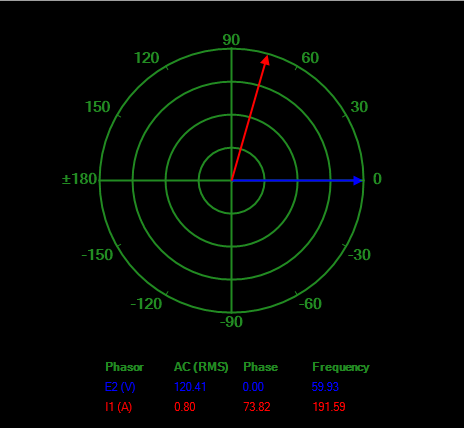
\includegraphics[width=0.75\textwidth]{figures/phasor-171.png}
	\end{center}
	\caption{}\label{fig1:}
\end{figure}

\begin{figure}[H]
	\begin{center}
		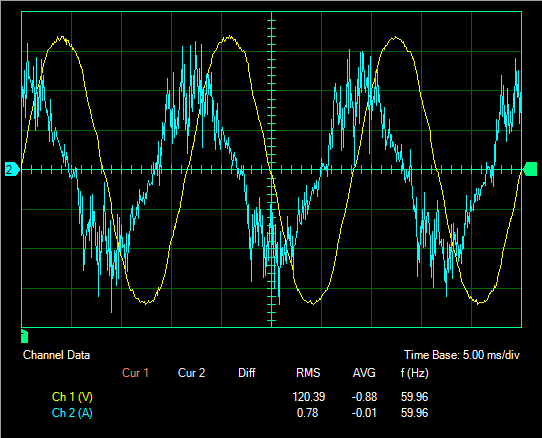
\includegraphics[width=0.75\textwidth]{figures/oscope-171.png}
	\end{center}
	\caption{}\label{fig2:}
\end{figure}

\begin{figure}[H]
	\begin{center}
		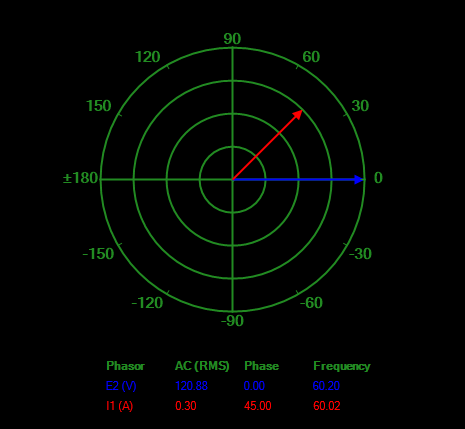
\includegraphics[width=0.75\textwidth]{figures/phasor-600.png}
	\end{center}
	\caption{}\label{fig3:}
\end{figure}

\begin{figure}[H]
	\begin{center}
		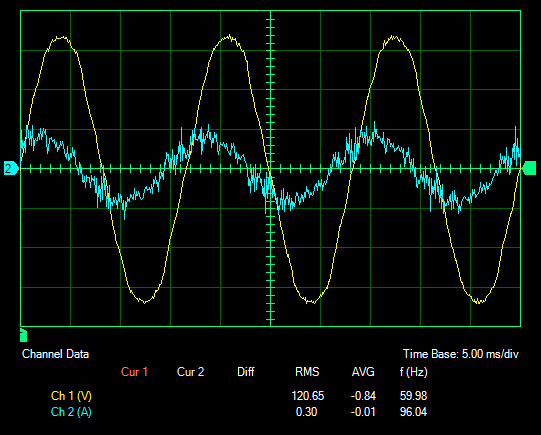
\includegraphics[width=0.75\textwidth]{figures/oscope-600.png}
	\end{center}
	\caption{}\label{fig4:}
\end{figure}

\begin{figure}[H]
	\begin{center}
		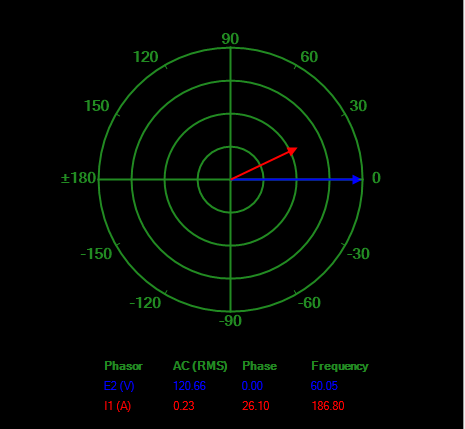
\includegraphics[width=0.75\textwidth]{figures/phasor-1200.png}
	\end{center}
	\caption{}\label{fig5:}
\end{figure}

\begin{figure}[H]
	\begin{center}
		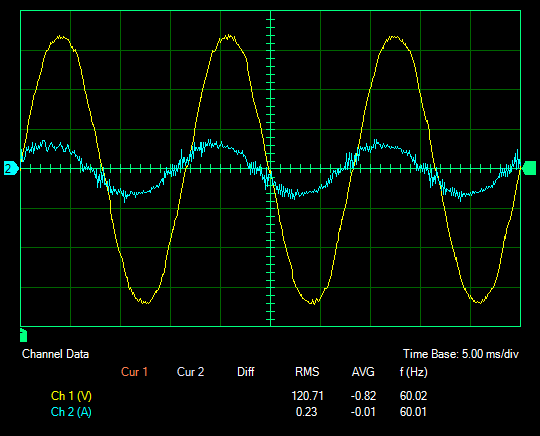
\includegraphics[width=0.75\textwidth]{figures/oscope-1200.png}
	\end{center}
	\caption{}\label{fig6:}
\end{figure}

\begin{figure}[H]
	\begin{center}
		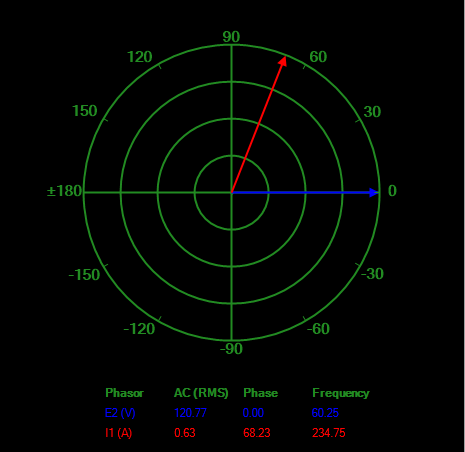
\includegraphics[width=0.75\textwidth]{figures/phasor-l-171.png}
	\end{center}
	\caption{}\label{fig7:}
\end{figure}

\begin{figure}[H]
	\begin{center}
		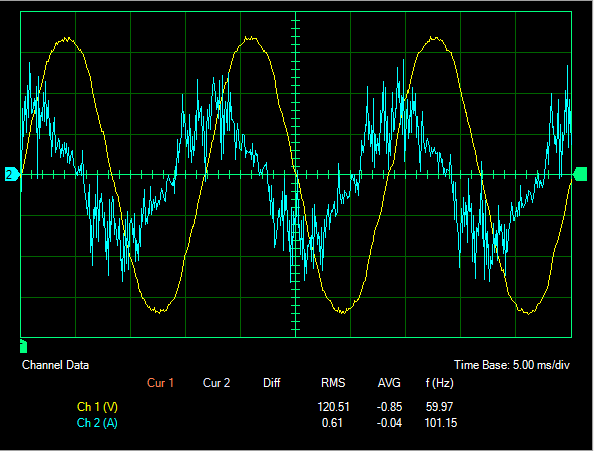
\includegraphics[width=0.75\textwidth]{figures/oscope-l-171.png}
	\end{center}
	\caption{}\label{fig8:}
\end{figure}

\begin{figure}[H]
	\begin{center}
		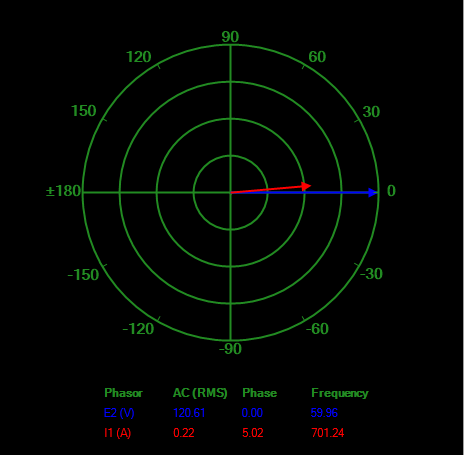
\includegraphics[width=0.75\textwidth]{figures/phasor-l-600.png}
	\end{center}
	\caption{}\label{fig9:}
\end{figure}

\begin{figure}[H]
	\begin{center}
		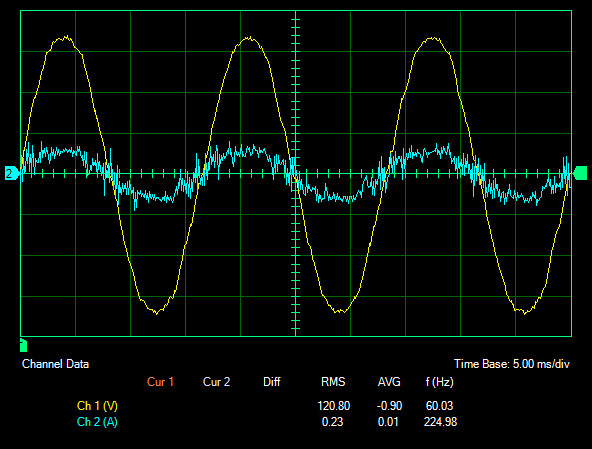
\includegraphics[width=0.75\textwidth]{figures/oscope-l-600.png}
	\end{center}
	\caption{}\label{fig10:}
\end{figure}

\begin{figure}[H]
	\begin{center}
		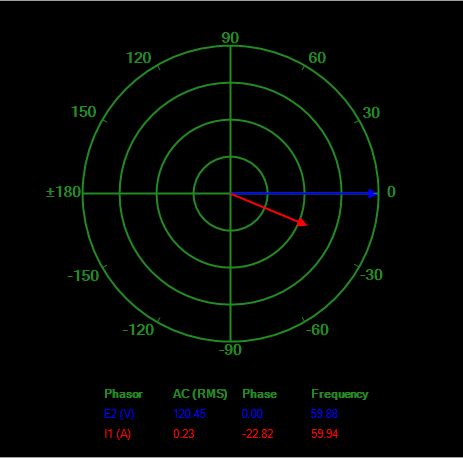
\includegraphics[width=0.75\textwidth]{figures/phasor-l-1200.png}
	\end{center}
	\caption{}\label{fig11:}
\end{figure}

\begin{figure}[H]
	\begin{center}
		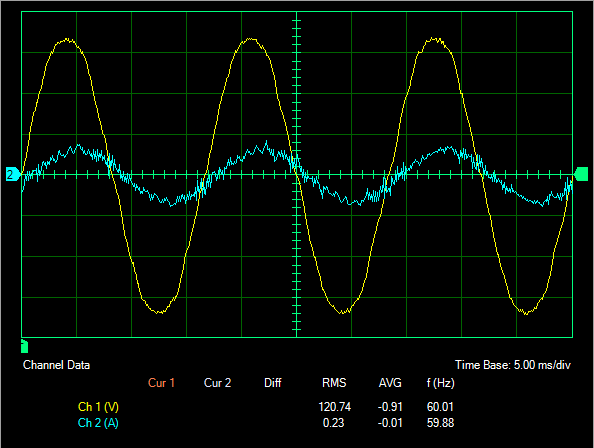
\includegraphics[width=0.75\textwidth]{figures/oscope-l-1200.png}
	\end{center}
	\caption{}\label{fig12:}
\end{figure}


\section{Conclusion}

\paragraph{}The main goal of this lab was to understand how power factor correction works and how adding
capacitors affects reactive power, power factor, and line current. By testing both resistive and inductive loads,
we saw how adding capacitance can either improve or worsen power factor.

\paragraph{}For the purely resistive load, adding capacitance decreased the power factor and increased line current
because the circuit already had a power factor of 1. For the inductive load, adding capacitors helped offset the inductive
reactive power. At -j600 Ω, the power factor approached 1, reducing line current by approximately 19\% without
significantly changing the real power consumed.

\paragraph{}We also encountered some measurement discrepancies, including an unexpected 30° phase shift caused
by the measurement software referencing $V_{LL}$ instead of $V_\phi$, along with one set of incorrectly recorded data.
Despite these issues, our results generally agreed with theoretical expectations.

\paragraph{}Overall, this lab demonstrated how properly balancing inductive and capacitive reactive power can reduce
line current and unnecessary loading on electrical equipment. It also showed why choosing the correct amount of capacitance
is important, since too much can actually make the power factor worse.

\end{document}
